\chapter{The Effects of Na$_{2}$O and SiO$_{2}$ on Liquid Phase Sintering of Bayer Al$_{2}$O$_{3}$}

\section{Introduction}
Al$_{2}$O$_{3}$ is arguably the most extensively used and researched ceramic material because it is used in many large volume applications such as high temperature refractories, technical ceramics, high voltage insulators, and functional fillers. The majority of Al$_{2}$O$_{3}$ applications use synthetic or specialty aluminas derived from Bayer feedstocks, such as aluminum trihydrate (Al(OH)$_{3}$), smelter grade Al$_{2}$O$_{3}$ and others. Bayer process aluminas are typically 99.0 - 99.9\% pure and contain Na$_{2}$O, CaO, Fe$_{2}$O$_{3}$, and SiO$_{2}$ impurities that originate from the bauxite ore and/or Bayer process reagents (e.g., NaOH). The vast majority of research on the sintering of Al$_{2}$O$_{3}$, however, focuses on ultra-high purity ($\geq$ 99.99\%) aluminas derived from specialty feedstocks, such as ammonium alum (NH$_{4}$Al(SO$_{4}$)$_{2}$$\cdot$12H$_{2}$O), boehmite ($\gamma$-AlOOH) and aluminum chloride (AlCl$_{3}$). While ultra-high purity aluminas provide the purest platform from which to conduct fundamental sintering research, that research does not usually explore the types and amounts of impurities typical of Bayer aluminas.  Commercial Bayer Al$_{2}$O$_{3}$ powders exist in a range of reactive grades that differ in the amount and types of these impurities. Therefore, the evaluation of specialty reactive aluminas, within the context of previous work on ultra-high purity aluminas, is a valuable contribution to industrial users and bridges fundamental sintering research with ultra-high purity aluminas.

\section{Experimental}

A chemically purified 0.4 $\mu$m median particle size Bayer process Al$_{2}$O$_{3}$ powder (Almatis, Inc., Leetsdale, PA, USA) with only 2 ppm MgO was used to study the sintering of near MgO-free Bayer Al$_{2}$O$_{3}$ (Figure \ref{Ch2-figure:Figure1}). The powder was chemically purified by the manufacturer so that impurity levels similar to commercial high purity Bayer process aluminas were obtained after doping with Na$_{2}$O and/or SiO$_{2}$. The physical and chemical characteristics of the as-received powder are shown in Table \ref{Ch2-table:table1}. Chemical analysis of the as-received Al$_{2}$O$_{3}$ was performed by inductively coupled plasma (ICP) emission spectroscopy (iCap 6000, Thermo Fischer Scientific, Inc., Waltham, MA, USA) after Al$_{2}$O$_{3}$ samples were acid digested in a microwave digestion unit in a Teflon$^{TM}$ sample holder.  It should be noted that the as-received Bayer Al$_{2}$O$_{3}$ contained impurity levels of 90 ppm Fe$_{2}$O$_{3}$, 62 CaO, and 22 ppm TiO$_{2}$.  The Na${2}$O and SiO$_{2}$ reported after doping include the impurity concentrations in the as-received powder (29 ppm Na$_{2}$O and 103 ppm SiO$_{2}$). 

The Al$_{2}$O$_{3}$ powders were doped with up to 1000 ppm Na$_{2}$O using sodium acetate (NaC$_{2}$H$_{3}$O$_{2}$$\cdot$3H$_{2}$O, ACS grade, BDH, West Chester, PA, USA), based on the procedure reported by Louet et al. \cite{Louet2005a}. The Al$_{2}$O$_{3}$ powders were dispersed in a solution of sodium acetate dissolved in de-ionized water. The suspension was stirred on a magnetic stir plate for 5 h at room temperature, and held at 80$^{\circ}$C for 24 h while stirring until the mixture was too viscous to stir, and then dried at 100$^{\circ}$C for 24 h. 

Samples were doped with up to 500 ppm SiO$_{2}$ by first dissolving tetraethyl orthosilicate (TEOS, Si(OC$_{2}$H$_{5}$)$_{4}$, 98\%, Aldrich Chemical Company, Inc., Milwaukee, WI, USA) in 200 proof ethanol with a few drops of de-ionized water to hydrolyze the TEOS and immediately mixed at room temperature for 5 h with either the as-received or Na$_{2}$O-doped Al$_{2}$O$_{3}$ powder. The mixture was subsequently stirred at 70$^{\circ}$C for an additional 12 h. The powder was then dried at 100$^{\circ}$C for 2 h, followed by crushing in a mortar and pestle, and sieving to -106 $\mu$m (US Standard 140 mesh).

Samples were prepared for sintering studies by uniaxially dry pressing the powders at 170 MPa and then cold isostatic pressing at 200 MPa (CIP, Autoclave Engineers, Erie, PA, USA) to obtain cylindrical samples (3.0-3.5 mm long by 12.7 mm diameter or 8.5-10 mm long by 6 mm diameter) with green densities of 59.0\% $\pm$ 0.5\% of theoretical density. To investigate the sintering process, dry pressed 8.5-10 mm long by 6 mm diameter cylinders were heated at 10$^{\circ}$C/min to 1525$^{\circ}$C in a thermomechanical analyzer (TMA, Linseis PT1600, Robbinsville, NJ, USA). The kinetics of sintering and grain growth were evaluated on 3.0-3.5 mm long by 12.7 mm diameter samples heated at 10$^{\circ}$C/min to 1200 $^{\circ}$C then 5$^{\circ}$C/min to 1525$^{\circ}$C followed by sintering at 1525$^{\circ}$C for up to 8 h. The density of three samples of each condition was measured by the Archimedes method according to ASTM standard B962-15 \cite{Standard2015} and the average density reported for each sintering time and temperature. For microstructure analysis, samples were first polished to a surface finish of 1 $\mu$m and then thermally etched in air at 1425$^{\circ}$C for 40 min. Average grain sizes were measured on SEM (ESEM, Quanta 200, FEI Company, Hillsboro, OR, USA) micrographs using a linear intercept method (ASTM Standard E112-96) \cite{Standard2013}.

\section{Results}

\subsection{Effects of Na$_{2}$O-doping}

The doping experiments were designed to uniformly distribute Na$_{2}$O and SiO$_{2}$ on the surfaces of the Al$_{2}$O$_{3}$ particles. Upon heating the dopant NaC$_{2}$H$_{3}$O$_{2}$$\cdot$3H$_{2}$O first dehydrates and then decomposes to form Na$_{2}$CO$_{3}$ above 385$^{\circ}$C \cite{Judd1974}. Using a video recorder, we observed that anhydrous sodium acetate melts and rapidly spreads on the surface of an Al$_{2}$O$_{3}$ substrate at $\sim$420$^{\circ}$C. Na$_{2}$CO$_{3}$ melts at 851$^{\circ}$C and subsequently decomposes to Na$_{2}$O \cite{Judd1974}. As a result of the rapid wetting of the Na$_{2}$O precursor on the Al$_{2}$O$_{3}$ substrate we conclude that Na$_{2}$O is uniformly distributed on the powder surface by the acetate doping process. 

Figure \ref{Ch2-figure:Figure2} shows the shrinkage behavior of Bayer Al$_{2}$O$_{3}$ doped with different Na$_{2}$O concentrations during heating to 1525$^{\circ}$C at 10$^{\circ}$C/min. The as-received Al$_{2}$O$_{3}$ (intrinsic impurities: 29 ppm Na$_{2}$O, 103 ppm SiO$_{2}$) begins to shrink at $\sim$1050 $^{\circ}$C, whereas shrinkage begins at 1100$^{\circ}$C for samples doped with 1029 ppm Na$_{2}$O. The difference in density at the beginning of densification continues throughout the heating cycle. However, above $\sim$1350$^{\circ}$C the densification rate of the Na$_{2}$O doped samples surpasses that of the as-received sample. Overall, the Na$_{2}$O-doped samples are 2.5\% less dense than the as-received Al$_{2}$O$_{3}$ after heating to 1525$^{\circ}$C.

Figure \ref{Ch2-figure:Figure3} shows the influence of Na$_{2}$O concentration on the densification kinetics at 1525$^{\circ}$C. Clearly, the degree of densification decreases with increasing Na$_{2}$O concentration for up to 30 min with the Na$_{2}$O-doped samples being as much as 2\% less dense than the as-received Al$_{2}$O$_{3}$. However, after $\geq$ 30 min at 1525$^{\circ}$C densification is independent of Na$_{2}$O content and all samples are 97.5-98.0\% dense after $\geq$ 3 h. 

The microstructures of as-received samples (29 ppm Na$_{2}$O) and samples doped with 529 ppm Na$_{2}$O sintered for 30 min, 3 h and 8 h at 1525$^{\circ}$C are compared in Figure \ref{Ch2-figure:Figure4}. It is seen that higher Na$_{2}$O concentration does not affect the average grain size for all hold times. Microstructures of as-received samples are predominantly equiaxed with a small number of facetted grains, whereas samples doped with Na$_{2}$O appear to have an increasing number of facetted grain boundaries with increasing Na$_{2}$O concentration. A few tabular grains of up to 60 $\mu$m were seen in both as-received and Na$_{2}$O-doped samples after 8 h at 1525$^{\circ}$C (see Figure \ref{Ch2-figure:Figure4}c and \ref{Ch2-figure:Figure4}f). Those facetted grains are larger in the as-received powder samples compared to Na$_{2}$O-doped samples, whereas the Na$_{2}$O-doped samples show more large tabular grains than samples from the as-received powder.

\subsection{Effects of Na$_{2}$O/SiO$_{2}$ co-doping}

As seen in Figure \ref{Ch2-figure:Figure5}, the presence of 603 ppm SiO$_{2}$ significantly retards densification of as-received alumina. Starting at $\sim$1250$^{\circ}$C, all of the SiO$_{2}$-doped samples densify less than as-received and singly Na$_{2}$O-doped samples. The densification rate of the SiO$_{2}$-doped samples from 1250 to 1525$^{\circ}$C is slower than the as-received alumina. SiO$_{2}$ reduces the linear shrinkage by $\sim$3.0\% and thus the samples are 8.7\% less dense than the as-received Al$_{2}$O$_{3}$ after 8 h at 1525$^{\circ}$C. 

The densification kinetics of the Al$_{2}$O$_{3}$ powders doped with different amounts of Na$_{2}$O (154 and 529 ppm) and SiO$_{2}$ (203 and 603 ppm) are compared in Figure \ref{Ch2-figure:Figure6}. It is seen that the addition of SiO$_{2}$ significantly reduces sintered density for all hold times. For example, samples containing as much as 603 ppm SiO$_{2}$ have densities of 81.5\% after 0 h and 93.8\% after 8 h at 1525$^{\circ}$C, whereas the as-received and singly Na$_{2}$O-doped Al$_{2}$O$_{3}$ samples are 98\% dense after 3 h at 1525$^{\circ}$C. 

Figure \ref{Ch2-figure:Figure6} shows the effect of Na$_{2}$O on the densification of SiO$_{2}$-doped samples. For hold times < 1 h, samples doped with 529 ppm Na2O and 203 ppm SiO2 are $\sim$ 1.5\% denser than samples doped with 154 ppm Na$_{2}$O and 203 ppm SiO$_{2}$. A difference in Na$_{2}$O concentration does not affect the final density of samples containing 203 ppm SiO$_{2}$ (96.5 - 97.0\%) after 3 h at 1525$^{\circ}$C. For higher SiO$_{2}$ concentrations (603 ppm), singly SiO$_{2}$ doped samples are 1 - 2.5\% less dense than samples co-doped with 529 ppm Na$_{2}$O and 603 ppm SiO$_{2}$ for all hold times at 1525$^{\circ}$C. 

The average grain sizes of the as-received and Na$_{2}$O-doped samples are nominally the same and increase from 1.6 $\mu$m to 2.5 $\mu$m after 30 min and 8 h at 1525$^{\circ}$C, respectively. There was little grain growth (1.4 $\mu$m to 2.1 $\mu$m) in singly SiO$_{2}$-doped samples (603 ppm) after 30 min and 8 h at 1525$^{\circ}$C, respectively. In samples co-doped with 529 ppm Na$_{2}$O and 603 ppm SiO$_{2}$ the average grain size is 1.6 $\mu$m for hold times between 30 min and 8 h at 1525$^{\circ}$C. The limited grain growth is attributed primarily to the large fraction of porosity. Micrographs of 603 ppm SiO$_{2}$ singly doped and 529 ppm Na$_{2}$O and 603 ppm SiO$_{2}$ co-doped samples heated for 8 h after heating for 8 h at 1525$^{\circ}$C are compared in Figure \ref{Ch2-figure:Figure7}. Both samples are only 92-94\% dense and thus it was difficult to prepare polished micrographs without some grain pull-out. 

\section{Discussion}

To understand the above effects, we first note from the Al$_{2}$O$_{3}$-Na$_{2}$O phase diagram \cite{Lambotte2013a} that Na$_{2}$O is insoluble in $\alpha$-Al$_{2}$O$_{3}$. A few platelet shaped grains with high aspect ratios were observed in the microstructures of sintered Na$_{2}$O-doped samples (Figure \ref{Ch2-figure:Figure8}). Due to their morphology and literature reports, \cite{Brownmiller1932a,PABLOGALAN1959,Rankin1916,Ridgway1936,Duncan1969a} it is assumed that these grains are a type of $\beta$-Al$_{2}$O$_{3}$. Four types of $\beta$-Al$_{2}$O$_{3}$ exist; two of them, $\beta$-Al$_{2}$O$_{3}$ (Na$_{2}$O$\cdot$11Al$_{2}$O$_{3}$) and $\beta$"-Al$_{2}$O$_{3}$ (Na$_{2}$O$\cdot$5Al$_{2}$O$_{3}$), form in the binary system Na$_{2}$O-Al$_{2}$O$_{3}$ \cite{Sutorik1998,Stevens1984}. The determination of which type of $\beta$-Al$_{2}$O$_{3}$ forms and the conditions of formation were not the subject of this work, so these analyses were not performed.

Sodium aluminate (NaAlO$_{2}$) is reported to form at temperatures as low as 900$^{\circ}$C,\cite{Christie1978} and $\beta$"-Al$_{2}$O$_{3}$ (Na$_{2}$O$\cdot$5Al$_{2}$O$_{3}$) can be synthesized at temperatures as low as 1100 $^{\circ}$C \cite{Brownmiller1932,Kummer1972,Vries1969}. Therefore, we hypothesize that either sodium aluminate or $\beta$"-Al$_{2}$O$_{3}$ forms before the onset of densification and that the presence of the second phases on the surface of the Al$_{2}$O$_{3}$ particles retards the initial shrinkage of Na$_{2}$O-doped samples at $\sim$1050$^{\circ}$C.  However, we did not observe any $\beta$-Al$_{2}$O$_{3}$ type grains in the samples at this temperature. Alternatively, as discussed below, Na$_{2}$O may interact with the 103 ppm of intrinsic SiO$_{2}$ in the sample.

We hypothesize that the initial grain boundaries in the as-received Al$_{2}$O$_{3}$ are wetted with the intrinsic impurities such as Na$_{2}$O, CaO, TiO$_{2}$ and SiO$_{2}$. Doping with Na$_{2}$O and SiO$_{2}$ changes the relative grain boundary chemistries and the properties of the respective grain boundary liquids. In the presence of a grain boundary liquid, densification occurs by a solution-precipitation sintering process, and thus, the rate of densification is controlled by either interface reaction between the grain boundary liquid and Al$_{2}$O$_{3}$ grains, or by the diffusion of Al$^{3+}$ through the liquid grain boundary film. Al$^{3+}$ diffusion is rate-limiting at 1525$^{\circ}$C since it has been shown for molten glass systems that Al$^{3+}$ has lower ionic diffusion rates than O$^{2-}$ \cite{Terai1975}. For diffusion-controlled densification, the densification rate is given by \cite{Kwon1990,Kwon1991}

%%
\begin{equation}
\label{Ch2-eq: diffusioncontrolled}
\frac{d\left( \frac{\Delta \rho}{\rho} \right)}{dt} = \frac{A \delta D_{l} C_{0} \gamma_{l \nu} \Omega}{kT} r_{s}^{-4}
\end{equation}
%%

\noindent and for interface reaction-controlled densification, the densification rate is given by 

%%
\begin{equation}
\label{Ch2-eq: interfacecontrolled}
\frac{d\left( \frac{\Delta \rho}{\rho} \right)}{dt} = \frac{B K C_{0} \gamma_{l \nu} \Omega}{kT} r_{s}^{-2}
\end{equation}
%%

\noindent where $A$ and $B$ are geometric factors, $\delta$ is the thickness of the liquid film, $D_{l}$ is the diffusion coefficient of Al$^{3+}$ in the liquid, $C_{o}$ is the equilibrium solute concentration, $K$ the interface reaction constant, $\gamma_{l \nu}$ is the liquid surface tension, $\Omega$ is the molecular volume of the solid, $r_{s}$ is the particle radius, $k$ is the Boltzmann constant and $T$ is absolute temperature.

Equations \ref{Ch2-eq: diffusioncontrolled} and \ref{Ch2-eq: interfacecontrolled} can be used to gain insights into the rate-limiting densification mechanisms during liquid phase sintering by evaluating their ratio \cite{Kwon1990,Kwon1991}

%%
\begin{equation}
\label{Ch2-eq: densmech}
\alpha = \frac{A \delta D_{l}}{BK}r_{s}^{-2}
\end{equation}
%%

In general, for $\alpha$ > 1, densification is controlled by the interface reaction, since $D_{l}$ is relatively high.  For $\alpha$ < 1, densification is controlled by diffusion, and for $\alpha$ = 1 both mechanisms contribute equally to densification \cite{Kwon1991}. Since the product of the grain boundary thickness and the diffusion coefficient greatly influences the rate-determining mechanism, $\delta D_{l}$ and the interface reaction constant $K$ were examined in more detail. 

Because the main impurities in Bayer aluminas are SiO$_{2}$ and Na$_{2}$O, the Al$_{2}$O$_{3}$-SiO$_{2}$-Na$_{2}$O ternary phase diagram \cite{Lambotte2013a} was utilized to evaluate the effects of dopant type and concentration on solubility of Al$_{2}$O$_{3}$ in the grain boundary liquid. It is assumed that the system approaches thermodynamic equilibrium upon holding at 1525$^{\circ}$C, and thus the equilibrium composition of the liquid at 1525$^{\circ}$C can be calculated from the ternary phase diagram (Figure \ref{Ch2-figure:Figure9}). For simplification, we considered only Al$_{2}$O$_{3}$, SiO$_{2}$ and Na$_{2}$O for the analysis, and assumed that all impurities/dopants are located in the grain boundaries. It was stated earlier that Na$_{2}$O is not soluble in Al$_{2}$O$_{3}$, and it has been reported in the literature that SiO$_{2}$ segregates at the grain boundaries in Al$_{2}$O$_{3}$ \cite{Park2000}. Figure \ref{Ch2-figure:Figure9} shows the liquidus projection of the Al$_{2}$O$_{3}$-SiO$_{2}$-Na$_{2}$O ternary phase diagram. The red solid lines connecting the Al$_{2}$O$_{3}$ end member to the Na$_{2}$O-SiO$_{2}$ side are binary cuts through the ternary (isoplethal sections) and correspond to some of the Na$_{2}$O/SiO$_{2}$ ratios investigated in this study. The red dashed line is the isotherm at 1525$^{\circ}$C for the part of the phase diagram where $\alpha$-Al$_{2}$O$_{3}$ and liquid are in equilibrium. The blue dash-dot line and the green dotted line are eutectic lines along which $\beta$-Al$_{2}$O$_{3}$ or mullite is stable with $\alpha$-Al$_{2}$O$_{3}$ and a liquid. The isotherm and the eutectic lines are important for determining the stable phases and the composition of the liquid in the samples. If a binary cut intersects the isotherm (red dashed line) only $\alpha$-Al$_{2}$O$_{3}$ and liquid are stable phases at 1525$^{\circ}$C and the intersection point determines the composition of the liquid. If a binary cut intersects one of the two marked eutectic lines (blue dash-dot or green dotted) a third phase ($\beta$-Al$_{2}$O$_{3}$ or mullite) is stable in those samples, and the composition of the liquid at 1525$^{\circ}$C is determined by the intersection point of the respective intersected eutectic line with the isotherm at 1525$^{\circ}$C.

The Al$_{2}$O$_{3}$-SiO$_{2}$-Na$_{2}$O phase diagram demonstrates that a small amount of liquid is stable at 1525$^{\circ}$C for all compositions investigated. Note that these overall compositions are all very close to the Al$_{2}$O$_{3}$ end member ($\sim$ 99.8\% Al2O3) and Na$_{2}$O and SiO$_{2}$ are insoluble in Al$_{2}$O$_{3}$. Isoplethal sections (red solid lines in Figure \ref{Ch2-figure:Figure9}) can be used to determine the stability and equilibrium composition of a liquid since the volume fractions of Na$_{2}$O and SiO$_{2}$ are known. Lambotte and Chartrand \cite{Lambotte2013a} calculated isoplethal sections of the ternary phase diagram, and based on their calculations, the solubility of Al$_{2}$O$_{3}$ in the liquid at 1525$^{\circ}$C in the samples was estimated based on the respective Na$_{2}$O:SiO$_{2}$ ratios (assuming a constant liquid density of 2.45 g/cm \cite{Standard2013,Day1962}). Likewise, the volume fractions of liquid and solid phases can be estimated since the doping and impurity concentrations of SiO$_{2}$ and Na$_{2}$O are known. Table \ref{Ch2-table:table2} summarizes the stable phases, the liquid compositions, and the total amount of liquid in the as-received and doped samples. Stable liquids at 1525$^{\circ}$C are predicted for liquid compositions with Na$_{2}$O:SiO$_{2}$ ratios between 0.25 and 0.5. As described above, for higher Na$_{2}$O concentrations in the samples (global Na$_{2}$O:SiO$_{2}$ ratio > 0.5), $\alpha$-Al$_{2}$O$_{3}$, $\beta$-Al$_{2}$O$_{3}$ and a liquid with a Na$_{2}$O:SiO$_{2}$ ratio of 0.5 are stable. For sample compositions with higher SiO$_{2}$ concentrations (global Na$_{2}$O:SiO$_{2}$ ratio < 0.25) $\alpha$-Al$_{2}$O$_{3}$, mullite and a liquid with a Na$_{2}$O:SiO$_{2}$ ratio of 0.25 are stable. Since the global Na$_{2}$O:SiO$_{2}$ ratio in most of the samples investigated in this work is either > 0.5 or < 0.25, the liquid in those samples had compositions of 0.5 or 0.25, respectively. As the Na$_{2}$O:SiO$_{2}$ ratio in the liquid increases from 0.25 to 0.5 the solubility of Al$_{2}$O$_{3}$ in the liquid increases from 18.4 vol.\% to 21.6 vol.\% \cite{Lambotte2013a}. The increased Al$_{2}$O$_{3}$ solubility leads to higher densification rates and higher densities in Na$_{2}$O/SiO$_{2}$ co-doped samples compared to singly SiO$_{2}$-doped samples, regardless of the rate-limiting process. 

Assuming fully dense samples and the liquid volume fractions reported in Table \ref{Ch2-table:table2}, we calculated the grain boundary thickness $\delta$ using:

%%
\begin{equation}
\label{Ch2-eq: gbthickness}
\delta = 2 \frac{V_{g} \phi}{S_{g} \left(1-\phi\right)}
\end{equation}
%%

\noindent where $\phi$ is the liquid volume fraction and $V_{g}$ and $S_{g}$ are the volume and the surface area based on the average grain size, respectively. For as-received and singly Na$_{2}$O-doped samples the grain boundary thickness is < 0.3 nm for all observed grain sizes. For Na$_{2}$O/SiO$_{2}$-co-doped samples (603 ppm SiO$_{2}$) the grain boundary thickness is between 0.8 and 1.8 nm for grain sizes of 1 $\mu$m and 2.5 $\mu$m, respectively. The calculated grain boundary thickness of singly SiO$_{2}$-doped samples is similar to that of as-received samples, since mullite is predicted to form in the Al$_{2}$O$_{3}$-SiO$_{2}$-Na$_{2}$O system for low Na$_{2}$O concentrations at 1525$^{\circ}$C. However, mullite may not form in Bayer process Al$_{2}$O$_{3}$ due to the presence of other impurities, such as CaO, which, similar to Na$_{2}$O, lowers the eutectic temperature and acts as a network modifier in the glass. Therefore, the grain boundary thicknesses of singly SiO$_{2}$-doped and Na$_{2}$O/SiO$_{2}$ co-doped samples are expected to be similar at $\sim$1.8 nm. The amount of liquid in the samples and, therefore, the grain boundary thickness, is governed mainly by the amount of glass forming species in the samples, i.e. SiO$_{2}$.

The diffusion coefficient of Al$^{3+}$ through the liquid grain boundary phase can be calculated with the Eyring relation

%%
\begin{equation}
\label{Ch2-eq: eyring}
D_{l} = \frac{kT}{\eta \lambda}
\end{equation}
%%

\noindent where $\eta$ is the viscosity of the grain boundary liquid and $\lambda$ is the jump distance of the diffusion species, taken as the ionic diameter of an Al$^{3+}$ (1.07 $\AA$). Using viscosity data (range of 20 - 400 Pa*s) from the literature \cite{Wu2015}, we estimated the diffusion coefficients to be $\sim$1*10$^{-7}$ and $\sim$5*10$^{-9}$ cm$^{2}$/s for Na$_{2}$O/SiO$_{2}$ co-doped and singly SiO$_{2}$-doped samples, respectively.

Although we can calculate values for grain boundary thickness ($\delta$) and viscosity ($\eta$), an exact $\alpha$-ratio cannot be determined using Equation \ref{Ch2-eq: densmech} because we do not know the interface reaction constant ($K$). Nevertheless, assuming a reasonable $K$ value from the literature ($K$ = 5*10$^{-8}$ m/s) \cite{Kwon1991} and assuming that the A/B ratio (A and B being geometrical factors) is on the order of 1, we estimated $\alpha$ to be $\sim$10$^{-2}$ and $\sim$1 for singly SiO$_{2}$-doped samples (603 ppm SiO$_{2}$) and Na$_{2}$O/SiO$_{2}$ co-doped samples (529/603 ppm), respectively. Thus, we conclude that at 1525$^{\circ}$C densification of Bayer aluminas with low Na$_{2}$O/SiO$_{2}$ concentration ratios is governed by diffusion, whereas densification of Bayer aluminas with high Na$_{2}$O/SiO$_{2}$ concentration ratios can be governed by either diffusion or interface reaction. 

The enhanced densification of Na$_{2}$O/SiO$_{2}$ co-doped samples compared to singly SiO$_{2}$-doped is attributed to two factors; the increased solubility of Al$_{2}$O$_{3}$ in the liquid grain boundary phase, and the enhanced diffusion of Al$^{3+}$ ($\sim$5*10$^{-9}$ to $\sim$1*10$^{-7}$ cm$^{2}$/s) through the liquid grain boundary. This effect of enhanced densification of Na$_{2}$O/SiO$_{2}$ co-doped samples compared to singly SiO$_{2}$-doped samples is observed in both the dilatometry curves and the densification kinetics data shown in Figure \ref{Ch2-figure:Figure2} and Figure \ref{Ch2-figure:Figure6}, respectively. 

It should be noted that a particular challenge for thermal processing studies with soda-based ceramics is Na$_{2}$O volatilization at relatively lower temperature than the sintering temperature. Soda by itself is highly volatile at temperatures < 1000$^{\circ}$C and the evaporation of soda from Na$_{2}$O containing technical ceramics such as sodium niobates \cite{Popovic2012} and $\beta$-Al$_{2}$O$_{3}$ during sintering is often reported. For example, $\beta$-Al$_{2}$O$_{3}$ (Na$_{2}$O$\cdot$11Al$_{2}$O$_{3}$) has an appreciable Na$_{2}$O vapor pressure at temperatures > 1400$^{\circ}$C \cite{Kummer1972}, and when heated in air to > 1500$^{\circ}$C, $\beta$-Al$_{2}$O$_{3}$ converts to $\alpha$-Al$_{2}$O$_{3}$ by volatilization of Na$_{2}$O \cite{Kummer1972,Gallup1935}. Therefore, Na$_{2}$O evaporation from the samples during heating should be considered as samples might have somewhat lower Na$_{2}$O concentrations than assumed for the above calculations. Thus, for samples with low Na$_{2}$O:SiO$_{2}$ ratios, the liquid grain boundary phase may contain somewhat less Na$_{2}$O and the grain boundary thickness may be somewhat less than calculated. However, for singly Na$_{2}$O-doped samples and for co-doped samples with high Na$_{2}$O:SiO$_{2}$ ratios (e.g. Na$_{2}$O $\geq$ 529 ppm for samples with 603 ppm SiO$_{2}$) the composition of the grain boundary liquid and the grain boundary thickness is not expected to change very much if Na$_{2}$O volatizes. Consequently, even with Na$_{2}$O volatilization, the proposed sintering mechanisms do not change. The evaporation of Na$_{2}$O from Bayer Al$_{2}$O$_{3}$ samples will be further discussed in future work.

\section{Summary}

High concentrations of Na$_{2}$O in Bayer process Al$_{2}$O$_{3}$ powders inhibit densification in the initial sintering stage and retard densification up to the final sintering stage compared to powders with low Na$_{2}$O concentrations. However, Na$_{2}$O shows no adverse effect on the final density after longer hold times ($\geq$ 3 h at 1525$^{\circ}$C). The addition of SiO$_{2}$ to Bayer process Al$_{2}$O$_{3}$ powders substantially retards densification, starting at $\sim$1250$^{\circ}$C, and samples containing as much as 603 ppm SiO$_{2}$ are 4\% less dense than samples containing 103 ppm SiO$_{2}$, even after hold times as long as 8 h at 1525$^{\circ}$C. Co-doping with Na$_{2}$O and SiO$_{2}$ increases densification by 1 - 2.5\% relative density relative to singly SiO$_{2}$-doped samples. The observed differences in sintering behavior can be explained by a liquid phase sintering model. Diffusion and solubility of Al$_{2}$O$_{3}$ in the SiO$_{2}$-based liquid in the grain boundaries is low at the temperatures used in this study, which explains the substantial retardation of densification by SiO$_{2}$. As predicted from the phase diagram Na$_{2}$O increases the solubility of Al$_{2}$O$_{3}$ in the siliceous grain boundary phase. As predicted from viscosity data Na$_{2}$O enhances diffusion of Al$^{3+}$ through the liquid grain boundary phase. Both factors contribute to the enhanced densification rates of samples with high Na$_{2}$O/SiO$_{2}$ ratios compared to samples with low Na$_{2}$O/SiO$_{2}$ ratios.

\newpage
\begin{table}[H]
	\caption{Physical and chemical characteristics of the as-received Bayer Al$_{2}$O$_{3}$ powder used in this study.}
	\centering
	\begin{tabular}{ | c | c | }
		\hline
		 & \\
		\hline
		BET (m$^{2}$/g) & 7.4 \\
		\hline
		D$_{50}$ ($\mu$m) & 0.4 \\
		\hline
		D$_{90}$ ($\mu$m) & 1.5 \\
		\hline
		 & ICP (ppm) \\
		\hline
		Al$_{2}$O$_{3}$ & 99.96 \% \\
		\hline
		SiO$_{2}$ & 103 \\
		\hline
		Na$_{2}$O (total) & 29 \\
		\hline
		Fe$_{2}$O$_{3}$ & 90 \\
		\hline
		CaO & 62 \\
		\hline
		TiO$_{2}$ & 22 \\
		\hline
		MgO & 2 \\
		\hline
	\end{tabular}
	\label{Ch2-table:table1}
\end{table}
\clearpage
%%%

\newpage
\begin{table}[H]
	\caption{Calculated compositions and amounts of liquid in as-received, singly doped and co-doped samples at 1525$^{\circ}$C ($\alpha$ = $\alpha$-Al$_{2}$O$_{3}$, $\beta$ = $\beta$-Al$_{2}$O$_{3}$, L = liquid, M = mullite).}
	\centering
	\resizebox{\textwidth}{!}{\begin{tabular}{ | c | c | c | c | c | c | c | c | c | }
		\hline
		\multicolumn{2}{|l|}{Global dopant} & Global & Na$_{2}$O:SiO$_{2}$ & \multicolumn{3}{l|}{Composition} & Amount & Stable \\
		\multicolumn{2}{|l|}{concentration} & Na$_{2}$O:SiO$_{2}$ & ratio in & \multicolumn{3}{l|}{of liquid} & of liquid & phases \\
		\cline{1-2}
		ppm (wt.) & ppm (mol) & ratio & Liquid & \multicolumn{3}{l|}{(mol \%)} & (vol. \%) & \\
		\cline{5-7}
		Na$_{2}$O/SiO$_{2}$ & Na$_{2}$O/SiO$_{2}$ & & & Na$_{2}$O & SiO$_{2}$ & Al$_{2}$O$_{3}$ & & \\
		\hline
		As-received & & & & & & & & \\
		29/103 & 48/175 & 0.27 & 0.25 & 17.9 & 63.4 & 19.7 & 0.03\% & $\alpha$+L \\
		\hline
		154/103- & 253/175- & & & & & & & \\
		1029/103 & 1693/175 & 1.45-9.67 & 0.5 & 26.1 & 52.3 & 21.6 & 0.03\% & $\alpha$+L+$\beta$ \\
		\hline
		29/603 & 48/1023 & 0.05 & 0.25 & 16.3  & 65.3 & 18.4 & 0.03\% & $\alpha$+L+M \\
		\hline
		154/603 & 253/1023 & 0.25 & 0.25 & 16.3 & 65.3 & 18.4 & 0.16\% & $\alpha$+L \\
		\hline
		279/603 & 459/1023 & 0.45 & 0.45 & 24.5 & 54.6 & 20.8 & 0.19\% & $\alpha$+L \\
		\hline
		529/603 & 870/1023 & 0.85 & 0.5 & 26.1 & 52.3 & 21.6 & 0.22\% & $\alpha$+L+$\beta$\\
		\hline
		1029/603 & 1693/1023 & 1.65 & 0.5 & 26.1 & 52.3 & 21.6 & 0.22\% & $\alpha$+L+$\beta$ \\
		\hline
	\end{tabular}}
	\label{Ch2-table:table2}
\end{table}
\clearpage
%%%

\newpage
%%%
\begin{figure}[H]
	\centering
	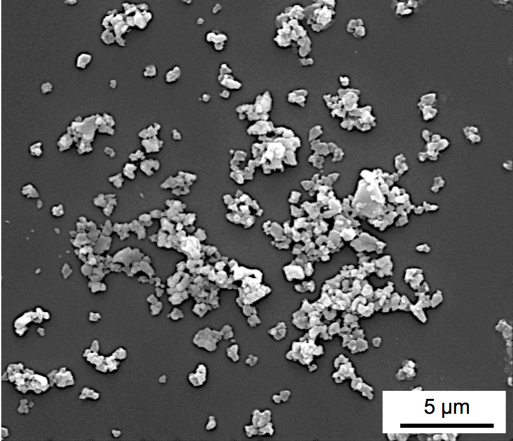
\includegraphics[width=\textwidth]{Chapter-2/Figures/Figure1.png}
	\caption{SEM image of as-received chemically purified Bayer Al$_{2}$O$_{3}$ powder used in this study.}
	\label{Ch2-figure:Figure1}
\end{figure}
%%%

\newpage
%%%
\begin{figure}[H]
	\centering
	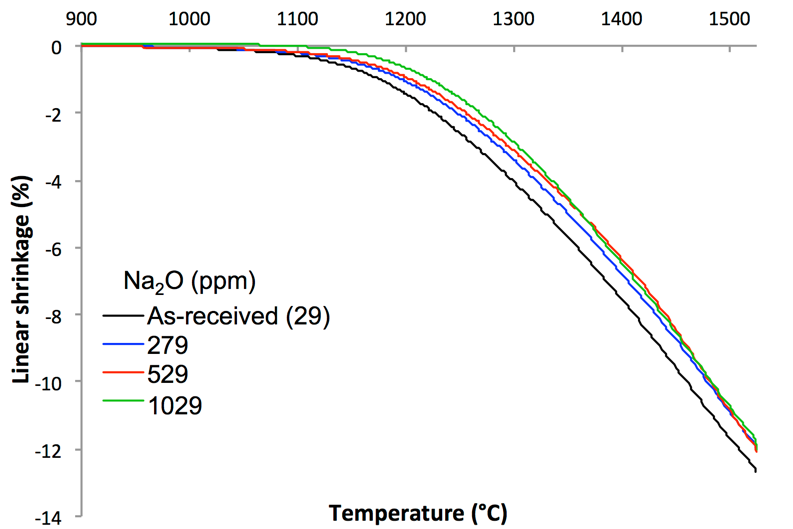
\includegraphics[width=\textwidth]{Chapter-2/Figures/Figure2.png}
	\caption{Dilatometer curves of as-received and singly Na$_{2}$O-doped samples heated at 10$^{\circ}$C/min to 1525$^{\circ}$C.}
	\label{Ch2-figure:Figure2}
\end{figure}
%%%

\newpage
%%%
\begin{figure}[H]
	\centering
	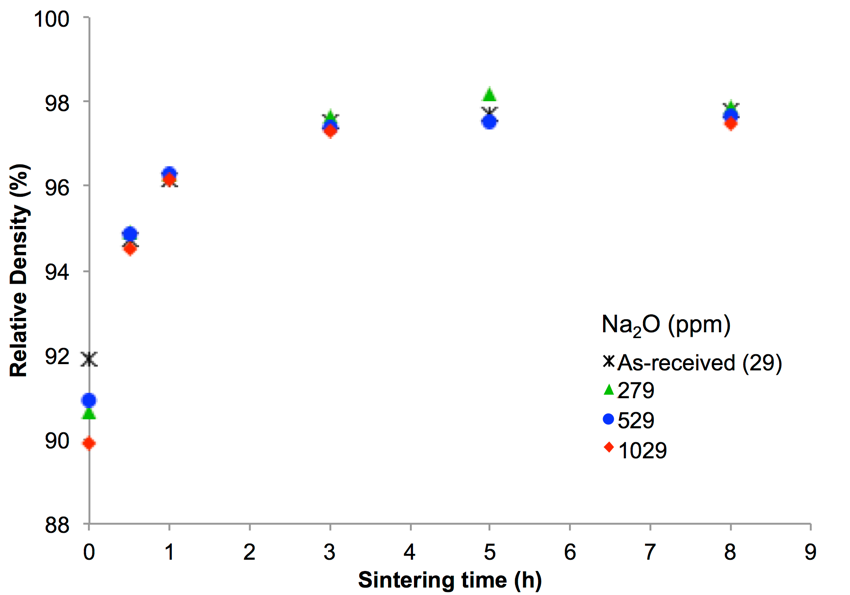
\includegraphics[width=\textwidth]{Chapter-2/Figures/Figure3.png}
	\caption{Densification kinetics of Bayer Al$_{2}$O$_{3}$ doped with different Na$_{2}$O concentrations and sintered at 1525$^{\circ}$C.}
	\label{Ch2-figure:Figure3}
\end{figure}
%%%

\newpage
%%%
\begin{figure}[H]
	\centering
	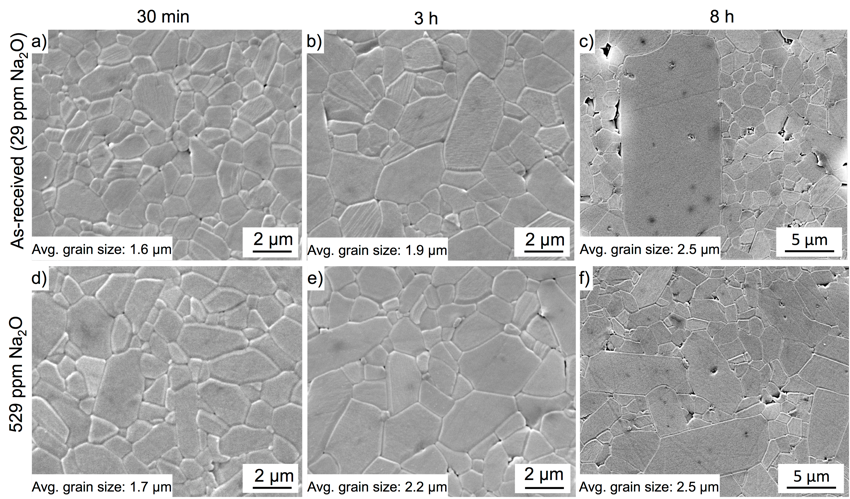
\includegraphics[width=\textwidth]{Chapter-2/Figures/Figure4.png}
	\caption{Microstructures of as-received and singly 529 ppm Na$_{2}$O doped samples after 30 min, 3 h and 8 h at 1525$^{\circ}$C.}
	\label{Ch2-figure:Figure4}
\end{figure}
%%%

\newpage
%%%
\begin{figure}[H]
	\centering
	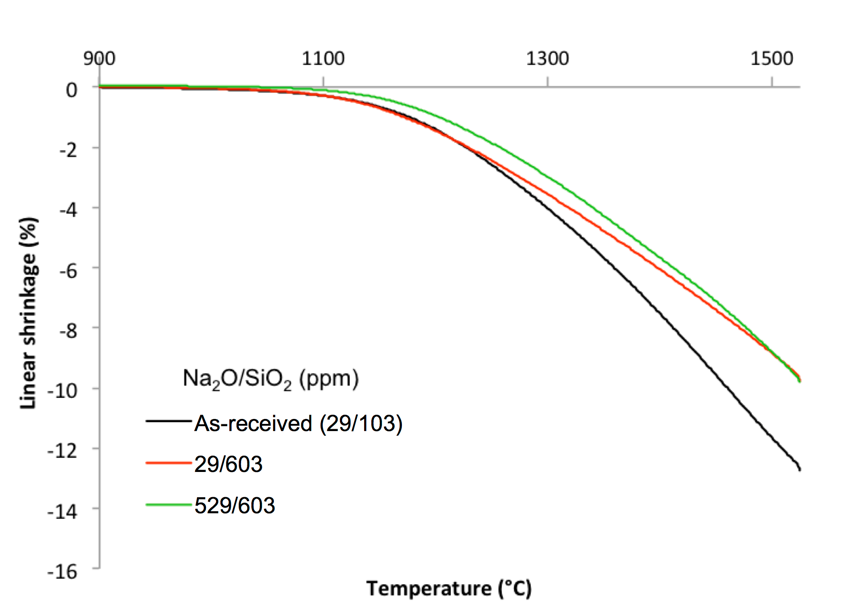
\includegraphics[width=\textwidth]{Chapter-2/Figures/Figure5.png}
	\caption{Dilatometer curves of as-received, singly SiO$_{2}$-doped, and Na$_{2}$O/SiO$_{2}$-doped Bayer Al$_{2}$O$_{3}$ heated at 10$^{\circ}$C/min to 1525$^{\circ}$C.}
	\label{Ch2-figure:Figure5}
\end{figure}
%%%

\newpage
%%%
\begin{figure}[H]
	\centering
	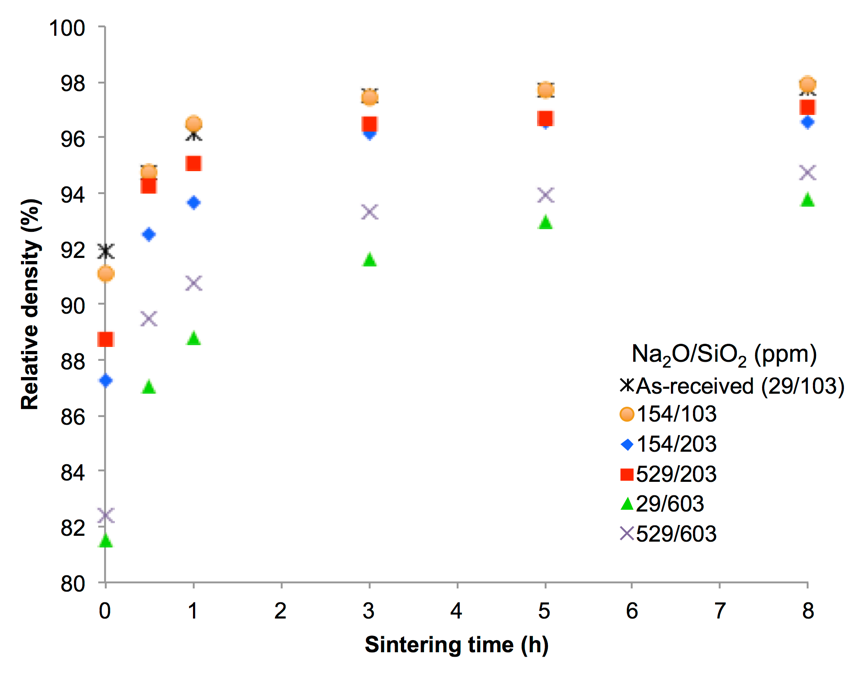
\includegraphics[width=\textwidth]{Chapter-2/Figures/Figure6.png}
	\caption{Densification kinetics of Bayer Al$_{2}$O$_{3}$ doped with different concentrations of Na$_{2}$O and SiO$_{2}$ at 1525$^{\circ}$C.}
	\label{Ch2-figure:Figure6}
\end{figure}
%%%

\newpage
%%%
\begin{figure}[H]
	\centering
	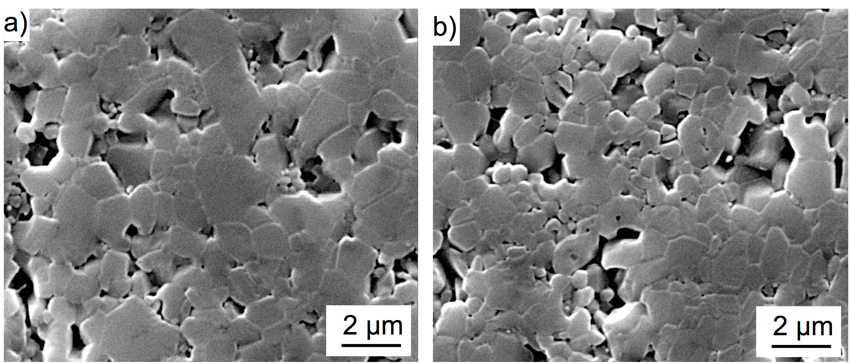
\includegraphics[width=\textwidth]{Chapter-2/Figures/Figure7.png}
	\caption{Microstructures of Bayer Al$_{2}$O$_{3}$ doped with a) 603 ppm SiO$_{2}$ and b) 529 ppm Na$_{2}$O and 603 ppm SiO$_{2}$ after heating at 1525$^{\circ}$C for 8h.}
	\label{Ch2-figure:Figure7}
\end{figure}
%%%

\newpage
%%%
\begin{figure}[H]
	\centering
	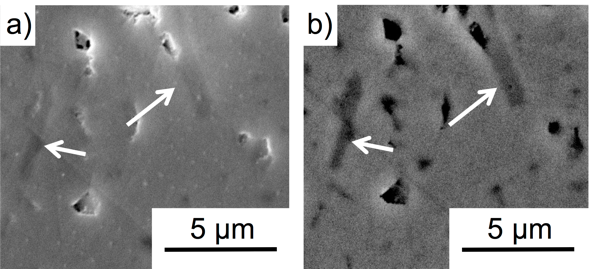
\includegraphics[width=\textwidth]{Chapter-2/Figures/Figure8.png}
	\caption{Micrographs of a sample doped with 1029 ppm Na$_{2}$O after sintering at 1525$^{\circ}$C for 3 h. The micrographs were recorded using a) a secondary electron detector and b) a backscattered electron detector. The arrows point at the platelet shaped $\beta$-alumina grains that form in samples doped with Na$_{2}$O. The samples were not thermally etched.}
	\label{Ch2-figure:Figure8}
\end{figure}
%%%

\newpage
%%%
\begin{figure}[H]
	\centering
	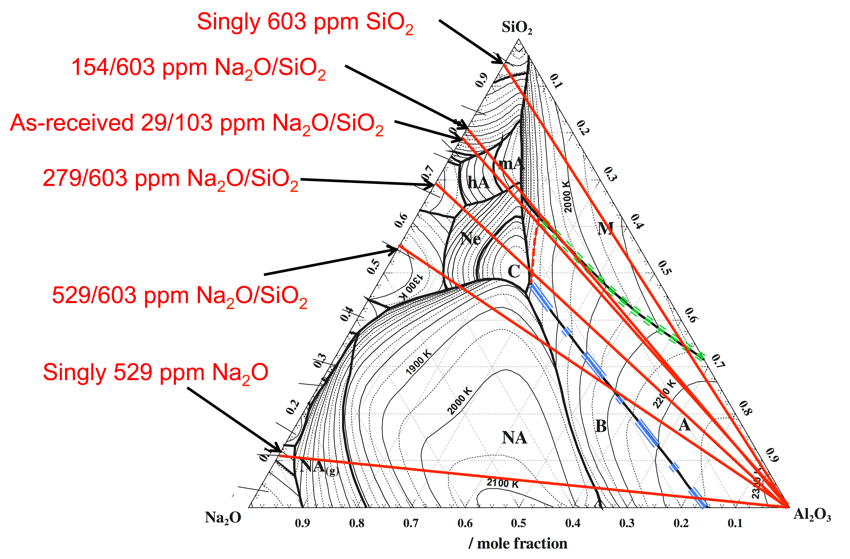
\includegraphics[width=\textwidth]{Chapter-2/Figures/Figure9.png}
	\caption{Liquidus projection of the Al$_{2}$O$_{3}$-SiO$_{2}$-Na$_{2}$O ternary phase diagram. The red solid lines are isoplethal cuts representing the samples investigated in this study. The red dashed line is the 1525$^{\circ}$C isotherm where $\alpha$-Al$_{2}$O$_{3}$ and liquid are in equilibrium. The blue dash-dot line and green dotted line are eutectic lines at which $\alpha$-Al$_{2}$O$_{3}$ and liquid is in equilibrium with $\beta$-Al$_{2}$O$_{3}$ or mullite, respectively.}
	\label{Ch2-figure:Figure9}
\end{figure}
%%%
